% This is part of Un soupçon de mathématique sans être agressif pour autant
% Copyright (c) 2013
%   Laurent Claessens
% See the file fdl-1.3.txt for copying conditions.

\begin{exercice}\label{exosmath-0339}

    Deux joueurs de jeu de combat tirent des rayons de plasma. Si les rayons s'intersectent, il se produit une explosion qui tue tout le monde dans un rayon de \unit{4}{\meter}. 


%The result is on figure \ref{LabelFigVMNerGf}. % From file VMNerGf
%\newcommand{\CaptionFigVMNerGf}{<+Type your caption here+>}

    \begin{multicols}{2}
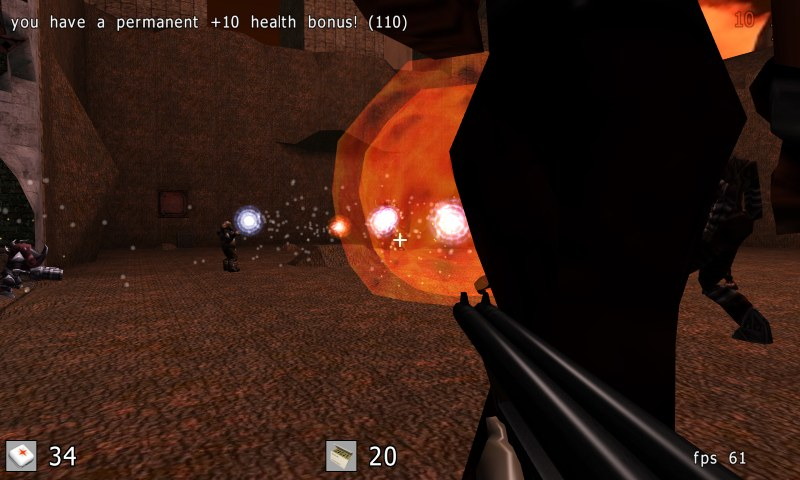
\includegraphics[width=10cm]{screenshot_5891783.png}\\
\href{http://sauerbraten.org/}{Capture d'écran de Cube 2}

\columnbreak

\input{Fig_VMNerGf.pstricks}

    \end{multicols}

    Si les joueurs \( A\) et \( B\) sont comme ci-dessus, vont-ils survivre ? Répondre par le calcul.

\corrref{smath-0339}
\end{exercice}
